\section{Архитектура CLaNN и её производные}

В рамках предложенного подхода CLaNN (Convex Laplace Neural Network)
энергия деформации \(\psi(\vect{\xi})\) с мерой деформации Лапласа аппроксимириуется посредством 
выпуклой по входу нейронной сетью (Input Convex Neural Network, ICNN) \cite{icnn2017}
и вычисления 2 тензора напряжения Пиолы-Кирхгофа \(\vect{S}\), используя явное выражение \eqref{eq:stress_components_2d}. 

\textbf{Обобщенная архитектура ICNN}

ICNN представляет собой класс нейронных сетей, гарантирующих выпуклость выходной функции относительно входных переменных. 
В нашем случае, функция энергии деформации $\psi: \mathbb{R}^3 \rightarrow \mathbb{R}$ называется выпуклой, 
если $\forall \vect{\xi}_1, \vect{\xi}_2 \in \mathbb{R}^3$ и $\lambda \in [0,1]$ выполняется неравенство Йенсена:
\begin{equation}
\psi(\lambda \vect{\xi}_1 + (1-\lambda) \vect{\xi}_2) \leq \lambda \psi(\vect{\xi}_1) + (1-\lambda) \psi(\vect{\xi}_2).
\label{eq:convexity_definition}
\end{equation}

Ключевые условия ICNN \cite{icnn2017}: 
(i) поэлементно выпуклая, монотонно неубывающая активация $\varphi$; 
(ii) $\mathbf{W}_z^{(\ell)}\!\ge\!0$ для всех слоёв 
(только на связях $z\!\to\!z$; $\mathbf{W}_x^{(\ell)}$, $\mathbf{b}^{(\ell)}$ без ограничений по знаку); 
(iii) каждый слой имеет прямую аффинную связь с входом 
$\boldsymbol{\xi}$: $z^{(\ell+1)}=\varphi\!\big(\mathbf{W}_z^{(\ell)}z^{(\ell)}+\mathbf{W}_x^{(\ell)}\boldsymbol{\xi}+\mathbf{b}^{(\ell)}\big)$; 
(iv) скалярный выход как $a^{\top} z^{(L)}+c$ с $a\!\ge\!0$ (или ещё один слой $\varphi$).

\textbf{Шаг 1. Однослойный ICNN и выбор активации.}
Рассмотрим однослойный вариант ICNN (с одним скрытым слоем) для аппроксимации $\psi(\boldsymbol{\xi})$:
\begin{equation}
  s = \mathbf{W}_1 \,\boldsymbol{\xi} + \mathbf{b}_1,\qquad
  z = \varphi_{\beta}(s),\qquad
  \tilde{\psi} = \mathbf{W}_2^{\top} z + b_2,\qquad \mathbf{W}_2 \ge 0.
  \label{eq:icnn_onelayer}
\end{equation}

\begin{equation}
  \varphi_{\beta}(x) = \frac{\operatorname{softplus}(\beta x)}{\beta},
  \label{eq:softplus_activation}
\end{equation}

Здесь $\varphi_{\beta}$ — выпуклая неубывающая функция активации \cite{dugas2001incorporating}, 
которая гладко аппроксимирует ReLU и при конечных $\beta$ является строго выпуклой; $\varphi_{\infty}(x)=\max(0,x)$.
Условие $\mathbf{W}_2\!\ge 0$ сохраняет выпуклость линейной комбинации. 
Размерности: $\mathbf{W}_1\!\in\mathbb{R}^{h\times 3}$, $\mathbf{b}_1\!\in\mathbb{R}^{h}$, 
$\mathbf{W}_2\!\in\mathbb{R}^{h}_{\ge 0}$, $h$ — размерность скрытого слоя.

\textbf{Шаг 2. Центрирование энергии $\psi$ в естественном состоянии.}
Для выполнения условия $\psi(\mathbf{0})=0$ центрируем энергию, 
вычитая значение нелинейной части при $\boldsymbol{\xi}=\mathbf{0}$:
\begin{equation}
  z_0 = \varphi_{\beta}(\mathbf{b}_1),\qquad
  \psi(\boldsymbol{\xi}) = \mathbf{W}_2^{\top}\big(z - z_0\big),\qquad (b_2 \equiv 0).
  \label{eq:center_psi}
\end{equation}
Тогда $\psi(\mathbf{0})=0$. Поскольку $z_0$ не зависит от $\boldsymbol{\xi}$, 
градиент $\partial\psi/\partial\boldsymbol{\xi}$ и гессиан $\partial^2\psi/\partial\boldsymbol{\xi}^2$ 
совпадают с таковыми для $\tilde{\psi}$, сохраняя выпуклость и гладкость.

\textbf{Шаг 3. Центрирование отклика $\mathbf{r}$ в естественной конфигурации.}
Для выполнения условия $\vect S(\vect I)=\vect 0$ обнулим линейный отклик в точке 
$\boldsymbol{\xi}=\mathbf{0}$:
\begin{equation}
  \mathbf{r}_0 := \frac{\partial \psi}{\partial \boldsymbol{\xi}}\bigg|_{\boldsymbol{\xi}=\mathbf{0}},\qquad
  \psi_{\mathrm{phys}}(\boldsymbol{\xi}) = \psi(\boldsymbol{\xi}) - \mathbf{r}_0^{\top}\boldsymbol{\xi}.
  \label{eq:phys_energy}
\end{equation}

Тогда $\psi_{\mathrm{phys}}(\mathbf{0})=0$ и $\mathbf{r}(\mathbf{0})=\mathbf{0}$, 
а по цепному правилу \eqref{eq:chain-rule} получаем $\mathbf{S}(\mathbf{I})=\mathbf{0}$. 
Вычитание линейного члена не меняет гессиан и сохраняет выпуклость. 
Так как $\mathbf{r}(\mathbf{0})=\mathbf{0}$, точка $\boldsymbol{\xi}=\mathbf{0}$ является минимумом 
$\psi_{\mathrm{phys}}$, и значит $\psi_{\mathrm{phys}}\ge 0$.

После получения $\psi_{\mathrm{phys}}$ автоматически вычисляются 
$\partial\psi/\partial\boldsymbol{\xi}$ средствами autodiff, реализованными в современных библиотеках для машинного обучения 
\cite{pytorch2019}, \cite{tensorflow2016}, \cite{jax2018}, 
после чего тензор напряжений $\mathbf{S}$ находится по формуле \eqref{eq:stress_components_2d} с 
использованием связи $\psi(\vect C)=\psi\big(\boldsymbol{\xi}(\vect C)\big)$.

Центрирование $\psi_{\mathrm{phys}}$ и $\mathbf{r}$ в естественном состоянии 
дает возможность гарантирования выполнения \eqref{eq:natural_state_stress} и
позволяет избежать дополнительных ограничений на параметры сети

% (заменено на TikZ-схему в рис.~\ref{fig:clann_arc})

\textbf{Аналитические выражения для производных энергии}

\textbf{Градиент энергии деформации}

Аналитическое дифференцирование функции энергии по переменным \(\xi\) даёт выражение для градиента:

\begin{equation}
 \vect{r} = \nabla_\xi \psi_{\mathrm{phys}} = \vect W_1^T \left( \vect W_2 \odot \sigma(\beta (\vect W_1 \vect \xi + \vect b_1)) \right) - \vect r_0,
\label{eq:energy_gradient}
\end{equation}
где $\sigma(x) = \frac{1}{1 + e^{-x}}$ - сигмоида, 
а операция $\odot$ обозначает поэлементное произведение (Hadamard product). 
Данное выражение демонстрирует, что градиент энергии является линейной комбинацией строк матрицы $\vect W_1^T$ с весами, 
определяемыми произведением выходных весов $\vect W_2$ и значений функции активации $\sigma(\beta (\vect W_1 \vect\xi + \vect b_1))$.

\textbf{Гессиан энергии деформации}

Вторые производные энергии по переменным \(\xi\) определяют гессиан, который имеет следующую аналитическую форму:

\begin{equation}
 H_{ij} = \sum_h \sigma'_h\,W_{2,h}\,W_{h,i}W_{h,j},
\label{eq:energy_hessian}
\end{equation}

где $\sigma' = \beta\,\sigma(1-\sigma)$ - производная сигмоиды, 
$\sigma=\operatorname{sigmoid}(\beta s)$, а $s=\vect W_1\xi+\vect b_1$.

\textbf{Материальная устойчивость и положительная определённость}

Из строгой выпуклости \(\psi(\xi)\) следует положительная определённость гессиана:
\begin{equation}
 \vect H = \frac{\partial^2\psi}{\partial\xi^2} > 0,
\label{eq:positive_hessian}
\end{equation}
что обеспечивает положительную определённость касательных модулей упругости 
$\mathbb{C} = \partial^2\psi/\partial\vect C^2$ через цепное правило дифференцирования. 
Это свойство важно для численной стабильности конечно-элементных расчётов, 
поскольку на практике улучшает сходимость метода Ньютона и отсутствие сингулярностей в матрице жёсткости.

\begin{figure}[H]
  \centering
  \resizebox{\textwidth}{!}{% ===== CLaNN: однослойная ICNN (наглядная архитектура) =====
\begin{tikzpicture}[
  font=\small, node distance=9mm and 14mm, >={Latex},
  box/.style={draw, rounded corners, align=center, minimum height=7mm, inner sep=2mm},
  block/.style={box, fill=green!6, text width=44mm},
  pin/.style={circle, draw, minimum size=6mm, fill=white},
  neur0/.style={circle, draw, minimum size=6mm, fill=white},
  neur/.style={circle, draw, minimum size=6mm, fill=white},
  title/.style={font=\bfseries},
  every fit/.style={draw, rounded corners, inner sep=3mm}
]

% Входы (лог‑лапласовы координаты)
\node[pin] (x1) {$\xi_1$};
\node[pin, below=6mm of x1] (x2) {$\xi_2$};
\node[pin, below=6mm of x2] (x3) {$\xi_3$};

% Аффинная проекция
\node[neur0, right=14mm of x1, yshift=12mm] (h11) {};
\node[neur0, right=14mm of x1] (h12) {};
\node[neur0, right=14mm of x1, yshift=-12mm] (h13) {};
\node[align=center, right=14mm of x1, yshift=-22mm] (vdots0) {$\vdots$};
\node[neur0, right=14mm of x1, yshift=-34mm] (h14) {};
\draw[->] (x1) -- (h11.west);
\draw[->] (x2) -- (h11.west);
\draw[->] (x3) -- (h11.west);
\draw[->] (x1) -- (h12.west);
\draw[->] (x2) -- (h12.west);
\draw[->] (x3) -- (h12.west);
\draw[->] (x1) -- (h13.west);
\draw[->] (x2) -- (h13.west);
\draw[->] (x3) -- (h13.west);
\draw[->] (x1) -- (h14.west);
\draw[->] (x2) -- (h14.west);
\draw[->] (x3) -- (h14.west);
% \node[block, above=2mm of h11, text width=36mm] (aff) {$s = W_1\,\xi + b_1$};
\node[block, above=2mm of h11, text width=60mm, inner sep=3mm] (soft) {$z_i = \mathrm{softplus}(\beta (W_1\,\xi + b_1))/\beta$};

% % Скрытый слой (softplus): три нейрона, троеточие и ещё один
% \node[neur, right=14mm of h12, yshift=12mm] (h1) {};
% \node[neur, right=14mm of h12] (h2) {};
% \node[neur, right=14mm of h12, yshift=-12mm] (h3) {};
% \node[align=center, right=14mm of h12, yshift=-22mm] (vdots1) {$\vdots$};
% \node[neur, right=14mm of h12, yshift=-34mm] (h4) {};
% \draw[->] (h11.east) -- (h1.west);
% \draw[->] (h12.east) -- (h2.west);
% \draw[->] (h13.east) -- (h3.west);
% \draw[->] (h14.east) -- (h4.west);
% % Блок активации над нейронами
% \node[block, above=2mm of h1, text width=36mm] (soft) {$z_i = \mathrm{softplus}(\beta (W_1\,\xi + b_1)/\beta$};

% Линейный выход (неотрицательные веса)
\node[block, right=22mm of h12, text width=42mm] (readout) {$\psi(\boldsymbol{\xi}) = \mathbf{W}_2^{\top}\big(z - z_0\big) - \mathbf{r}_0^{\top}\boldsymbol{\xi}$};
\draw[->] (h11.east) -- (readout.west);
\draw[->] (h12.east) -- (readout.west);
\draw[->] (h13.east) -- (readout.west);
\draw[->] (h14.east) -- (readout.west);

% % Центрирование \to физическая энергия
% \node[block, below=10mm of readout] (psiphys) {$\psi_{\mathrm{phys}}(\boldsymbol{\xi}) = \psi(\boldsymbol{\xi}) - \mathbf{r}_0^{\top}\boldsymbol{\xi}$ \\
%   \scriptsize $r_0 = W_1^{\top}\!(w_2^{+}\!\odot\!\sigma(\beta b_1))$};
% \draw[->] (readout.south) -- (psiphys.north);

% Рамка и заголовок
\node[fit=(x1)(x3)(soft)(readout), label={[title]above:{Архитектура CLaNN: однослойная ICNN}}] (archfit) {};

\end{tikzpicture}}
  \caption{Схема архитектуры CLaNN.}
  \label{fig:clann_arc}
  \label{fig:clann_icnn1_nn}
\end{figure}

\begin{figure}[H]
  \centering
  \resizebox{\textwidth}{!}{% ======= CLaNN: FE stretch -> dataset -> CLaNN arch (vertical) -> S -> Train -> (g,H) -> FE inflation =======
% Требует: \usepackage{tikz} \usetikzlibrary{arrows.meta,positioning,fit}
\begin{tikzpicture}[
  font=\small, node distance=8mm and 14mm, >={Latex},
  box/.style={draw, rounded corners, align=center, minimum height=8mm, inner sep=2mm},
  thinbox/.style={draw, rounded corners, align=center, minimum height=6mm, inner sep=1.2mm, text width=52mm},
  inpin/.style={circle, draw, minimum size=5.2mm},
  hid/.style={circle, draw, minimum size=6mm},
  title/.style={font=\bfseries},
  dashedarrow/.style={->, dashed},
  boxL/.style={box, fill=blue!6},
  boxM/.style={box, fill=green!6},
  boxR/.style={box, fill=orange!10},
  trainbox/.style={box, fill=purple!8}
]

% ---------------- Simplified pipeline (3 columns, orthogonal arrows) ----------------
% LEFT COLUMN
\node[boxL, minimum width=46mm, minimum height=32mm] (fe) {FE-растяжение\\ \scriptsize протоколы $p$\\[2pt]
  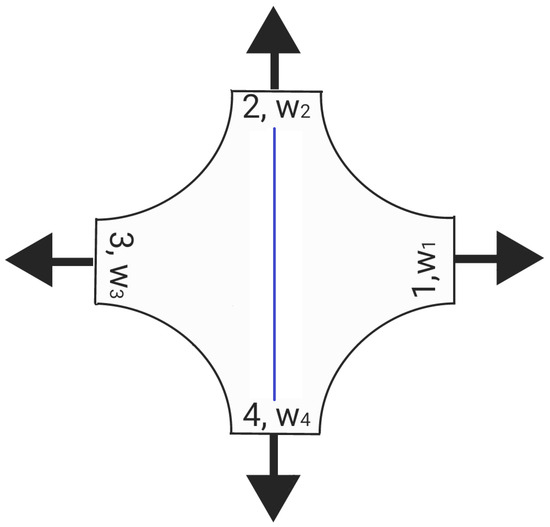
\includegraphics[width=0.3\linewidth]{img/malt_dirichlet.png}};
\node[boxL, below=8mm of fe, minimum width=46mm] (data) {Сбор данных\\ $D(p,w)=\{(C,S)\}$};

% MIDDLE COLUMN
\node[boxM, right=28mm of fe, minimum width=54mm] (xi) {деформация Лапласа\\ $\boldsymbol{\xi}=\boldsymbol{\xi}(C)$};
\node[boxM, below=8mm of xi, minimum width=54mm] (arch) {Архитектура CLaNN\\ $\psi_{\rm phys}(\boldsymbol{\xi})$};
\node[boxM, below=8mm of arch, minimum width=54mm] (smap) {Автодифференцирование \\ $S=\partial\psi/\partial C$};
\node[trainbox, below=8mm of smap, minimum width=54mm] (train) {Обучение\\ $L=\|\vect S_{pred}-\vect S\|_{L2}$ (Adam)};

% RIGHT COLUMN
\node[boxR, right=28mm of arch, minimum width=50mm] (gh) {Производные\\ $g(\xi),\ H(\xi)$};
\node[boxR, below=8mm of gh, minimum width=50mm, minimum height=36mm] (infl) {FE-раздутие\\ рексация + Ньютон\\[2pt]
  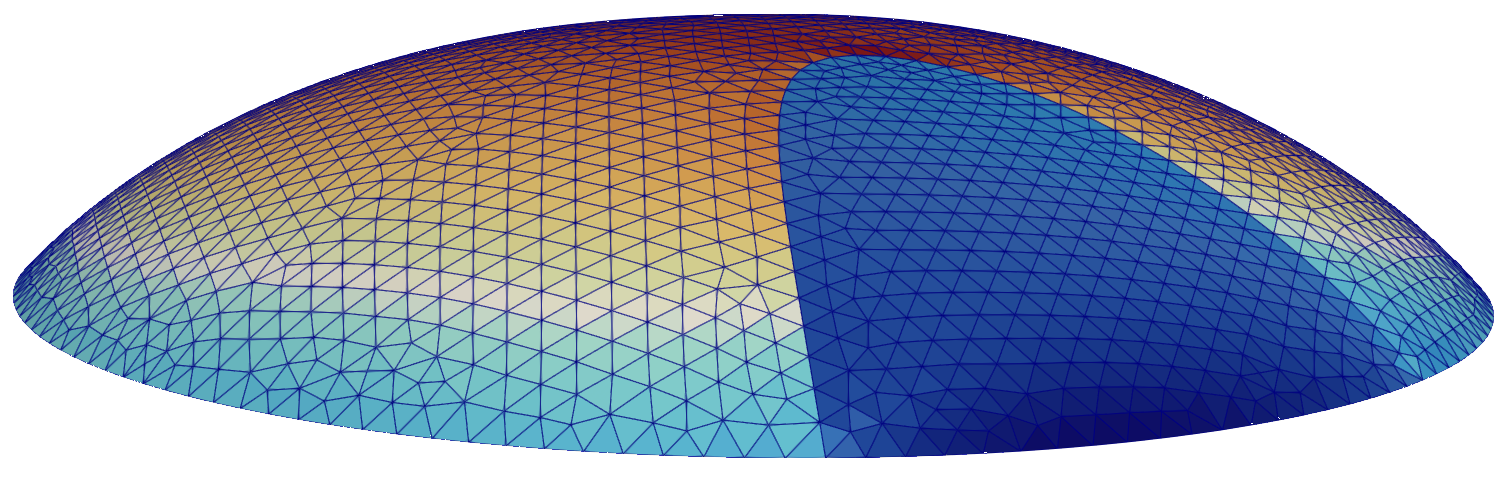
\includegraphics[width=0.3\linewidth]{img/Numerical/het/plane.png}};

% ORTHOGONAL ARROWS
\draw[->] (fe) -- (data);
% вилка от датасета: одна ветвь к деформации, другая — к обучению
\path (data.east) -- ++(10mm,0) coordinate (datasplit);
\draw[->] (data.east) -- (datasplit) |- (xi.west);
\draw[->] (datasplit) |- (train.west);
\draw[->] (xi) -- (arch);
\draw[->] (arch) -- (smap);
\draw[->] (smap) -- (train);
\draw[->] (arch.east) -- (gh.west);
\draw[->] (gh.south) -- (infl.north);
% пунктир: обновление параметров из обучения обратно в архитектуру (слева)
\draw[dashedarrow] (train.west) -- ++(-8mm,0) |- (arch.west);

\end{tikzpicture}
}
  \caption{Схема вычислительного контура CLaNN.}
  \label{fig:clann_pipeline}
\end{figure}

Такое построение архитектуры CLaNN обеспечивает выполнение всех необходимых физических свойств гиперупругой модели: 
\textbf{термодинамическая корректность} достигается через строгое соблюдение соотношения \eqref{eq:chain-rule}, 
что гарантирует консервативность напряжений $\oint \vect{S}:\mathrm{d}\vect{C} = 0$ и согласованность с законами 
термодинамики; 
\textbf{материальная устойчивость} обеспечивается и существенно улучшается за счёт строгой выпуклости функции энергии 
$\psi(\boldsymbol{\xi})$, гарантируемой архитектурой ICNN ($\vect{W}_2 \ge 0$, выпуклая неубывающая активация); 
\textbf{объективность} автоматически выполняется благодаря параметризации через тензор 
Коши-Грина $\vect{C} = \vect{F}^{\top}\vect{F}$, обеспечивая инвариантность относительно поворотов и симметрию напряжений; 
\textbf{строгая неотрицательность и коэрцитивность энергии} обеспечиваются архитектурной калибровкой 
$\psi_{\mathrm{phys}}(\boldsymbol{\xi}) = \mathbf{W}_2^{\top}(z - z_0) - \mathbf{r}_0^{\top}\boldsymbol{\xi}$,
что даёт $\psi_{\mathrm{phys}}(\mathbf{0})=0$, $\psi_{\mathrm{phys}}(\boldsymbol{\xi})>0$ при $\boldsymbol{\xi}\ne\mathbf{0}$ и 
$\psi_{\mathrm{phys}}(\boldsymbol{\xi})\to\infty$ при $\|\boldsymbol{\xi}\|\to\infty$; 
наконец, \textbf{физические ограничения} \eqref{eq:energy_constraints} обеспечиваются архитектурой сети CLaNN: монотонные, выпуклые функции активации,
неотрицательные весовые коэффициенты, центрирование энергии деформации $\psi$ и отклика $\vect r$.


